\documentclass[11pt]{beamer}
\usetheme{CambridgeUS}
\usepackage[utf8]{inputenc}
\usepackage[english]{babel}
\usepackage{amsmath}
\usepackage{amsfonts}
\usepackage{amssymb}
\usepackage{xcolor}
\newcommand{\todo}{\textcolor{red}{\textbf{TODO:}}}
\newcommand{\dof}[1]{\begin{itemize}
\item[-]\textcolor{blue}{\textbf{#1 DOFs}}
\end{itemize}}
\newcommand{\norm}[1]{\parallel{#1}\parallel}
\newcommand{\R}{\mathbb{R}}
\newcommand{\diff}[2]{\frac{\partial{#1}}{\partial{#2}}}

\author[Stefano, Marco]{Stefano De Filippis \& Marco Menchetti}
\title[ROB2 project]{Task priority assignment with collision avoidance}
%\setbeamercovered{transparent} 
%\setbeamertemplate{navigation symbols}{} 
\logo{
\includegraphics[scale=.1]{./images/logo.jpeg}}
\institute[Sapienza]{Sapienza - University of Rome} 
\date{} 
\subject{Robotics II} 
\begin{document}

\begin{frame}
\titlepage
\end{frame}

%\begin{frame}
%\tableofcontents
%\end{frame}

\begin{frame}{Why priority?}
\begin{itemize}
\item Decomposition of problems in many tasks.
\item Most problems \textcolor{red}{can't} be solved by just one task.
\item Error is kept on the tasks that \textcolor{red}{can't} be executed	\textbf{EXACTLY} 
\item More natural and smoother behavior.
\end{itemize}
\end{frame}

\begin{frame}{Collision avoidance. How?}
\begin{columns}
\begin{column}{.5\textwidth}
\begin{block}{1. Control points}
We push constantly the control point away from the obstacle so as to be sure they will never get in contact!
\textbf{\textcolor{red}{How do we handle priority?}}
\begin{itemize}
\item When the control point is too near the priority lowers (i.e. becomes more important)
\item As soon as the distance exit the \emph{dangerous} region the priority rise again
\end{itemize}
\end{block}
\end{column}
\begin{column}{.5\textwidth}
\todo Figure of the KUKA and its control points
\end{column}
\end{columns}
\end{frame}

\begin{frame}{Collision avoidance. How?}
\begin{columns}
\begin{column}{.5\textwidth}
\begin{block}{2. How do we push?}
We change approach whether the control point is on the e-e or on the structure:
\begin{itemize}
\item For the end-effector we add a cartesian velocity pointing away from the obstacle
\item For the ones on the structure we add assign a cartesian velocity projected along the distance from the obstacle (\textcolor{red}{1 DOF}).
\end{itemize}
\end{block}
\end{column}
\begin{column}{.5\textwidth}
\todo figure of the repulsive velocity
\end{column}
\end{columns}
\end{frame}

\begin{frame}{Tasks}
We know why to prioritize Tasks, but which are the ones we are going to use?
\begin{itemize}
\item[\textbf{1}] A cartesian positioning task (i.e. we want our e-e to behave in a certain way)
\dof{3}
\item[\textbf{2}] An orientation task used to simulate any kind of auxiliary task
\dof{1}
\item[\textbf{3,4}] Two collision avoidance task, each one on 1 DOF
\dof{2}
\end{itemize}
In the end we saturated 6 out of all the 7 DOFs of the manipulator.
\end{frame}

\begin{frame}{Task 1: Cartesian positioning}
\begin{columns}
\begin{column}{.5\textwidth}
Cartesian positioning means we want the end effector to execute a given trajectory  in $\Bbb R^3$.

\begin{block}{Path used:}
\begin{itemize}
\item A linear path
\item A circular path 
\end{itemize}
\end{block}

The associated jacobian $J_1$ is the analytical jacobian of the direct kinematics.
\end{column}
\begin{column}{.5\textwidth}
\todo pic
\end{column}
\end{columns}
\end{frame}

\begin{frame}{Task 1: Collision avoidance}
\begin{columns}
\begin{column}{.5\textwidth}
\begin{itemize}
\item We have \textbf{4} tasks occupying \textbf{6} DOF and we can't another cartesian positioning task. How is it performed?
\end{itemize}
\begin{block}{IDEA:}
Add another repulsive velocity to the desired one, pointing away from the obstacle! 
\end{block}
\begin{itemize}
\item In this way the \emph{Flacco Matrix} will handle the \textcolor{red}{exact} joint velocities so as to execute the \textcolor{red}{sum} of the two.
\item This won't change the jacobian of the task.
\end{itemize}
\end{column}
\begin{column}{.5\textwidth}
\todo pic
\end{column}
\end{columns}
\end{frame}

\begin{frame}{Repulsive velocity}
\begin{columns}
\begin{column}{.5\textwidth}
\begin{block}{How do we choose?}
We want the repulsive velocity to satisfy a certain amount of properties:
\begin{itemize}
\item Maximum admissible cartesian velocity at distance $d=0$ from the obstacle $\rightarrow V_{max}$.
\item Smooth descending curve $\rightarrow \alpha$.
\item Zero velocity after a given distance from the obstacle $\rightarrow \rho$.
\end{itemize}
\end{block} 
Hence:
\[
v(P,O) = \frac{V_{max}}{1+e^{(\norm{D(P,O)}(2\/\rho)-1)\alpha}}
\]
\end{column}
\begin{column}{.5\textwidth}
\todo right $v_{max}$
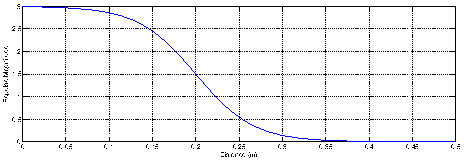
\includegraphics[scale=.75]{./images/repulsive_velocity.pdf}
\end{column}
\end{columns}
\end{frame}

\begin{frame}{Task 2: Link orientation}
The "orientation task" tries to keep constant the elevation of the third link axis. We need to define it as a vector in $\R^3$:
\[
p_l(q) = p_5(q) - p_4(q)
\]
Applying a coordinate transformation into spherical ones we can easily get the expression of the elevation (dropping the dependencies on $q$):
\[
\phi = \mathrm{arccos}(\frac{p_{l,z}}{\norm{p_l}})
\]
Denoting $p = \frac{p_{l,z}}{\norm{p_l}}$ we can get the expression of the associated jacobian as:
\[
\dot{\phi} = \diff{\phi}{p}\diff{p}{q}\dot{q}
\]
\end{frame}

\begin{frame}{Tasks 3,4: Control points}
\begin{columns}
\begin{column}{.5\textwidth}
We chose the following:
\begin{itemize}
\item \todo
\item \todo
\end{itemize}
\end{column}
\begin{column}{.5\textwidth}
\todo pic
\end{column}
\end{columns}
\end{frame}

\begin{frame}{Tasks 3,4: Collision avoidance}
As already introduced we can't perform collision avoidance for the control points using all the three component of the distance vector. \textcolor{red}{So what?}
\begin{columns}
\begin{column}{.5\textwidth}
\begin{block}{PROJECT!}
We can project the same repulsive velocity we used on task 1, on the distance from the obstacle, obtaining a "repulsive speed" we will call $v$ \todo check on report.
\end{block}
\end{column}
\begin{column}{.5\textwidth}
\begin{equation*}
v = \eta^T\dot{r_{o}} = \eta^T J_i\dot{q} = J_{c,i}\dot{q}
\end{equation*}
$J_i$ is the jacobian at the i-th control point.
\end{column}
\end{columns}
\end{frame}

\begin{frame}{Code}

\end{frame}

\begin{frame}{Results}

\end{frame}

\end{document}